% pdflatex
\documentclass[12pt]{article}
\usepackage{ebgaramond}
\usepackage{graphicx}
\usepackage{microtype}

\title{The Myth of Er\footnote{Excerpted from book \textsc{x} of the
\textit{Republic.} The main body of text is translated by Benjamin Jowett, but
all numbered footnotes are by Thomas Taylor. Some of these are translations of
Proclus' commentary upon the text. The editor has made minor changes to both
text and notes to reconcile the prose of the two authors.}}
\author{Plato (tr.~Benjamin Jowett)\footnote{B.~Jowett. \textit{The Republic
of Plato.} Clarendon Press, 1888.} \and Thomas Taylor\footnote{T.~Taylor.
\textit{The Works of Plato,} vol.~\textsc{i}.  R.~Wilkes, 1804.}}
\date{}

\begin{document}
\maketitle

\noindent I will tell you a tale; not one of the tales which Odysseus tells to
the hero Alcinous, yet this too is a tale of a hero, Er the son of Armenius, a
Pamphylian by birth. He was slain in battle, and ten days afterwards, when the
bodies of the dead were taken up already in a state of corruption, his body was
found unaffected by decay, and carried away home to be buried. And on the
twelfth day, as he was lying on the funeral pile, he returned to
life\footnote{In the manuscript Commentary of Proclus on this book of the
Republic, five examples are given of persons that have revived after they have
been for many days dead. That part of the Commentary containing these examples
is preserved by Alexander Morus, in his \textit{Not{\ae} ad qu{\ae}dam Loca
Novi F{\oe}deris,} which, as the book is scarce, I shall present to the public,
for the sake both of the learned and unlearned English reader.

Proclus then, after having observed that some in his time have been seen
sitting or standing on the sepulchers in which they had been buried, which,
says he, is also related by the ancients of Aristeas, Hermodorus, and
Epimenides, subjoins the following example, taken from the History of
Clearchus, the disciple of Aristotle: ``Cleonymus, the Athenian, who was a man
fond of hearing philosophic discourses, on the death of one of his associates,
becoming very sorrowful, and giving himself up to despair, apparently died, and
was laid out according to custom. His mother, as she was folding him in her
embraces, taking off his garment, and kissing him, perceived in him a gentle
breathing, and being extremely joyful on the occasion, delayed his burial.
Cleonymus in a short time after was restored to life, and told all that he saw
and heard when he was in a separate state. He said that his soul appeared, as
if liberated from certain bonds, to soar from its body, and that, having
ascended above the earth, he saw in it places all-various, both for their
figure and color, and streams of rivers unknown to men. And that at last he
came to a certain region sacred to Vesta, which was under the direction of
d{\ae}moniacal powers in indescribable female forms.''

The second example is from the historian Naumachius, ``who flourished (says
Proclus) in the time of our ancestors, and is on one Polycritus, who was an
illustrious and principal man among the {\AE}tolians. This Polycritus died, and
returned to life in the ninth month after his death; came to the general
assembly of the {\AE}tolians, and joined with them in their consultations about
what measures were best to be adopted. Hiero the Ephesian, and other
historians, testify the truth of this, in that account of transactions which
they send to king Antigonus, and their other absent friends.''

The third is as follows: ``In Nicopolis also (says Proclus), not long since,
the same thing happened to one Eurynous. This man, who was buried before the
city, revived fifteen days after, and said that he saw and heard many wonderful
things under the earth, which he was ordered not to relate. He lived some time
after this, and his conduct was more just after his revival than before.''

The fourth is of Rufus, a priest of the Thessalonians, who lived near the time
of the historian Naumachius. This man was restored to life the third day after
his death, for the purpose of performing certain sacred ceremonies, which he
had promised to perform, and, having fulfilled his promise, again died.

The fifth and last is of one Philon{\ae}a, who lived under the reign of Philip.
``She was the daughter (says Proclus) of Demostratus and Charite, who lived in
Amphipolis, and died soon after her marriage to one Craterus. She revived,
however, in the sixth month after her death, and, through her love of a youth
named Machates, who came to Demostratus from his own country Pelle, had
connection with him privately for many nights successively. This amour,
however, being at length detected, she again died; previous to which she
declared, that she acted in this manner according to the will of terrestrial
d{\ae}mons. Her dead body was seen by every one, lying in her father's house;
and on digging the place, which prior to this had contained her body, it was
seen to be empty, by those of her kindred who came thither, through unbelief of
what had happened to her. The truth of this relation is testified both by the
epistles of Hipparchus and those of Arrid{\ae}us, to Philip, in which they give
an account of the affairs of Amphipolis.''

Proclus then with his usual sagacity observes, concerning the cause of this
phenomenon, as follows: ``Many other of the ancients have collected a history
of those that have apparently died, and afterwards revived; and among these
are, the natural philosopher Democritus, in his writings concerning Hades, and
that wonderful Conotes, the familiar of Plato. [...]{\footnotemark} For the
death was not, as it seemed, an entire desertion of the whole life of the body,
but a cessation, caused by some blow, or perhaps a wound. But the bonds of the
soul yet remained rooted about the marrow, and the heart contained in its
profundity the empyreuma of life; and this remaining, it again acquired the
life which had been extinguished, becoming adapted to animation.''

Lastly, Proclus adds: ``That it is possible for the soul to depart from, and
enter into the body, is evident from him, who, according to Clearchus, used a
soul-attracting wand, on a sleeping lad, and who persuaded the d{\ae}moniacal
Aristotle, as Clearchus relates in his Treatise on Sleep, that the soul may be
separated from the body, and that it enters into the body, and uses it as a
lodging. For, striking the lad with the wand, he drew out, and as it were led
his soul, for the purpose of evincing that the body was immoveable when the
soul was at a distance from it, and that it was preserved uninjured. The soul
being again led into the body, by means of the wand, after its entrance related
every particular. From this circumstance, therefore, both other spectators, and
Aristotle, were persuaded that the soul is separate from the body.''} and told
them what he had seen in the other world. He said that when his soul left the
body he went on a journey with a great company,\footnotetext{There is an
unfortunate chasm here in the manuscript, of two or three lines.} and that they
came to a mysterious place at which there were two openings in the earth; they
were near together, and over against them were two other openings in the heaven
above. In the intermediate space there were judges seated, who commanded the
just, after they had given judgment on them and had bound their sentences in
front of them, to ascend by the heavenly way on the right hand; and in like
manner the unjust were bidden by them to descend by the lower way on the left
hand; these also bore the symbols of their deeds, but fastened on their backs.
He drew near, and they told him that he was to be the messenger who would carry
the report of the other world to men, and they bade him hear and see all that
was to be heard and seen in that place. Then he beheld and saw on one side the
souls departing at either opening of heaven and earth when sentence had been
given on them; and at the two other openings other souls, some ascending out of
the earth dusty and worn with travel, some descending out of heaven clean and
bright. And arriving ever and anon they seemed to have come from a long
journey, and they went forth with gladness into the meadow, where they encamped
as at a festival; and those who knew one another embraced and conversed, the
souls which came from earth curiously enquiring about the things above, and the
souls which came from heaven about the things beneath. And they told one
another of what had happened by the way, those from below weeping and sorrowing
at the remembrance of the things which they had endured and seen in their
journey beneath the earth (now the journey lasted a thousand years), while
those from above were describing heavenly delights and visions of inconceivable
beauty. The story would take too long to tell; but the sum was this:---He said
that for every wrong which they had done to any one they suffered tenfold; or
once in a hundred years---such being reckoned to be the length of man's life,
and the penalty being thus paid ten times in a thousand years. If, for example,
there were any who had been the cause of many deaths, or had betrayed or
enslaved cities or armies, or been guilty of any other evil behaviour, for each
and all of their offences they received punishment ten times over, and the
rewards of beneficence and justice and holiness were in the same proportion. I
need hardly repeat what he said concerning young children dying almost as soon
as they were born. Of piety and impiety to gods and parents, and of murderers,
there were retributions other and greater far which he described. He mentioned
that he was present when one of the spirits asked another, ``Where is
Ardi{\ae}us the Great?'' (Now this Ardi{\ae}us lived a thousand years before
the time of Er: he had been the tyrant of some city of Pamphylia, and had
murdered his aged father and his elder brother, and was said to have committed
many other abominable crimes.) The answer of the other spirit was: ``He comes
not hither and will never come. And this,'' said he, ``was one of the dreadful
sights which we ourselves witnessed. We were at the mouth of the cavern, and,
having completed all our experiences, were about to reascend, when of a sudden
Ardi{\ae}us appeared and several others, most of whom were tyrants; and there
were also besides the tyrants private individuals who had been great criminals:
they were just, as they fancied, about to return into the upper world, but the
mouth, instead of admitting them, gave a roar, whenever any of these incurable
sinners or some one who had not been sufficiently punished tried to ascend; and
then wild men of fiery aspect,\footnote{By these, d{\ae}mons of a punishing
characteristic are signified.} who were standing by and heard the sound, seized
and carried them off; and Ardi{\ae}us and others they bound head and foot and
hand, and threw them down and flayed them with scourges, and dragged them along
the road at the side, carding them on thorns like wool, and declaring to the
passers-by what were their crimes, and that they were being taken away to be
cast into hell.'' And of all the many terrors which they had endured, he said
that there was none like the terror which each of them felt at that moment,
lest they should hear the voice; and when there was silence, one by one they
ascended with exceeding joy. These, said Er, were the penalties and
retributions, and there were blessings as great.

\begin{figure}
\centering
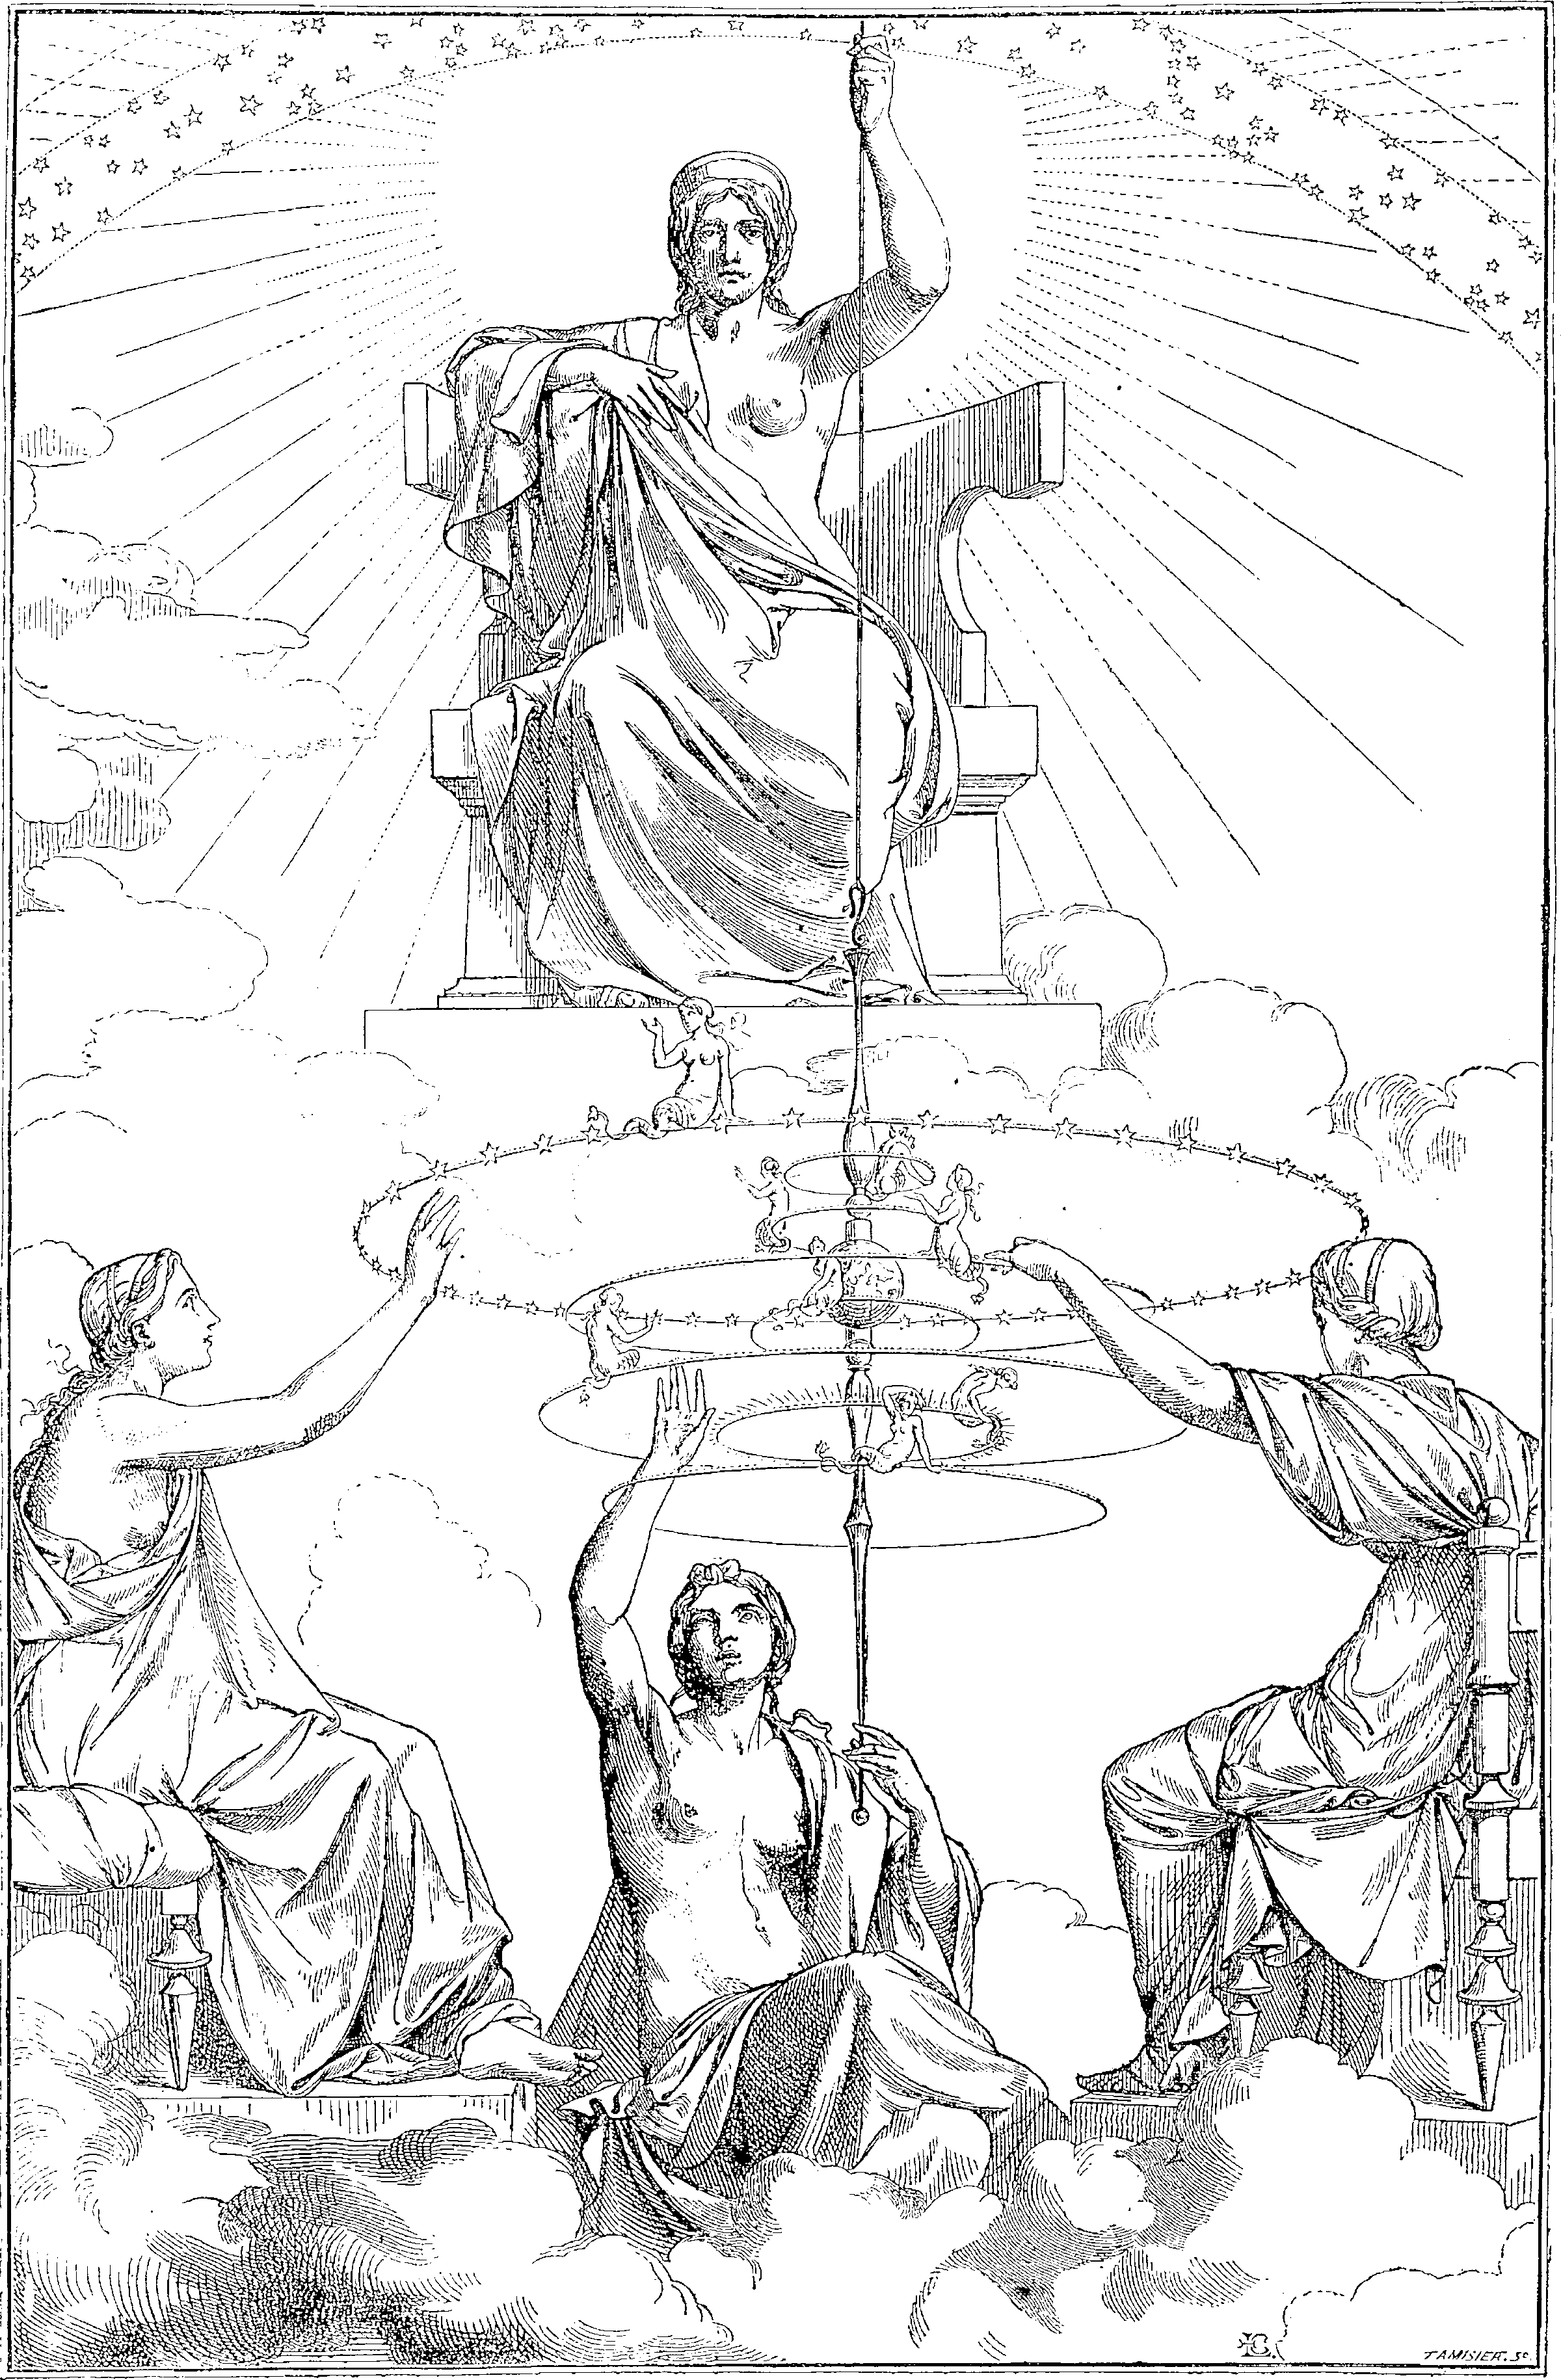
\includegraphics[width=\textwidth,totalheight=\textheight,keepaspectratio]{plato_myth_of_er.png}
\end{figure}

Now when the spirits which were in the meadow had tarried seven days, on the
eighth they were obliged to proceed on their journey, and, on the fourth day
after, he said that they came to a place where they could see from above a line
of light, straight as a column, extending right through the whole heaven and
through the earth, in color resembling the rainbow, only brighter and purer;
another day's journey brought them to the place, and there, in the midst of the
light, they saw the ends of the chains of heaven let down from above: for this
light is the belt of heaven, and holds together the circle of the universe,
like the under-girders of a trireme. From these ends is extended the spindle of
Necessity, on which all the revolutions turn. The shaft and hook of this
spindle are made of steel, and the whorl is made partly of steel and also
partly of other materials. Now the whorl is in form like the whorl used on
earth; and the description of it implied that there is one large hollow whorl
which is quite scooped out, and into this is fitted another lesser one, and
another, and another, and four others, making eight in all, like vessels which
fit into one another; the whorls show their edges on the upper side, and on
their lower side all together form one continuous whorl. This is pierced by the
spindle, which is driven home through the centre of the eighth. The first and
outermost whorl has the rim broadest, and the seven inner whorls are narrower,
in the following proportions---the sixth is next to the first in size, the
fourth next to the sixth; then comes the eighth; the seventh is fifth, the
fifth is sixth, the third is seventh, last and eighth comes the second. The
largest [or fixed stars] is spangled, and the seventh [or sun] is brightest;
the eighth [or moon] colored by the reflected light of the seventh; the second
and fifth [Saturn and Mercury] are in color like one another, and yellower
than the preceding; the third [Venus] has the whitest light; the fourth [Mars]
is reddish; the sixth [Jupiter] is in whiteness second. Now the whole spindle
has the same motion; but, as the whole revolves in one direction, the seven
inner circles move slowly in the other, and of these the swiftest is the
eighth; next in swiftness are the seventh, sixth, and fifth, which move
together; third in swiftness appeared to move according to the law of this
reversed motion the fourth; the third appeared fourth and the second fifth. The
spindle turns on the knees of Necessity; and on the upper surface of each
circle is a siren, who goes round with them, hymning a single tone or note. The
eight together form one harmony; and round about, at equal intervals, there is
another band, three in number, each sitting upon her throne: these are the
Fates,\footnote{In order to understand what is here delivered by Plato
respecting the Fates, it is necessary to observe that there is an order of Gods
immediately above those of a mundane characteristic, which was denominated by
ancient theologists liberated, and supercelestial. The peculiarity of this
order is represented to us by Plato, in what he now says concerning the Fates.
``In this place, therefore (says Proclus), Plato instructing us in the order of
the universe, which supernally pervades through the whole of mundane natures,
from the inerratic sphere, and in that order which governs human life, at
different times proposing elections of different lives, and varying the measure
of justice adapted to them, he refers the primary cause of this order to a
monad and triad exempt from mundane wholes. And to the monad he ascribes an
inspective government, extending its dominion at the same time to all heaven,
and represents it as being impartibly present with all things, as governing all
things indivisibly, and according to one energy, and as moving wholes with its
most subordinate powers. But to the triad he assigns a progression from the
monad, an energy proceeding into the universe, and a divisible fabrication. For
that which is simple and united in the exempt providence of the monad is
produced into multitude, through the secondary inspection of the triad.

``The one cause, therefore, (i.~e.~the monad) possesses more authority that the
triadic multitude. For all the variety of powers in the world, the infinity of
motions, and the multiform difference of reasons, is convolved by the triad of
the Fates; and this triad is again extended to one monad prior to the three,
which Socrates calls necessity, not as governing wholes by violence, nor as
obliterating the self-motive nature of our life, nor as deprived of intellect
and the most excellent knowledge, but as comprehending all things
intellectually, and introducing bound to things indefinite, and order to things
disordered. It is likewise so called by Socrates, as causing all things to be
obedient to its government, and extending them to the good, as subjecting them
to demiurgic laws, and guarding all things within the world, and as circularly
comprehending every thing in the universe, and leaving nothing void of the
justice which pertains to it, nor suffering it to escape the divine law.

``With respect to the order in which the Fates are arranged, it appears from
Plato in the \textit{Laws}, that the first is Lachesis, the second Clotho, and
the third Atropos. And here it must be diligently observed, that Socrates uses
the parts of time as symbols of comprehension according to cause. For that
which \textit{was}, was once future and the present, and that which now
\textit{is}, was once future; but the future is not yet the past, but has the
whole of its essence in becoming the future. These three causes, therefore, or
the three Fates, are analogous to these three portions of time: and of these,
the most perfect, and which comprehends the others, is that which sings the
past; for the past, having once been both the present and the future, may be
considered as comprehending these. The next to this in perfection is the
\textit{present}, which partly comprehends, and is partly comprehended; for it
comprehends the future, and is comprehended in the past. But the third is the
future, which is comprehended both in the past and the present; the latter
unfolding, and the former bounding, its progression. Hence Lachesis is the
primary cause, comprehending in herself the others; and Clotho is allotted a
superior, but Atropos an inferior order. And on this account Lachesis moves
with both her hands, as in a greater and more total degree, giving completion
to the more partial energies of the other two. But Clotho turns the spindle
with her right hand, and Atropos with her left, so far as the former precedes
with respect to energy, but the latter follows, and, in conjunction with the
former, governs all things. For in mortal animals the right hand is the
principle of motion; and in the wholes of the universe the motion to the right
hand comprehends that to the left.

``Observe too, that as it was before said that the whole spindle is turned on
the knees of Necessity, so the fable suspends the providence about partial
souls from the knees of Lachesis, who, with her hands, as with her more
elevated powers, perpetually moves the universe, but possesses with subjection
in her knees the causes of the periods of souls.

``In the next place, let us consider the symbols with which the fable
celebrates their dominion. Their walking then in the celestial circles
signifies their exempt and separate government. But their being seated on
thrones, and not in the circles themselves, like the Sirens, indicates that the
receptacles which are first illuminated by them are established above the
celestial orbs. For a throne is the vehicle and receptacle of those that are
seated on it: and this perspicuously signifies that these divinities are
proximately placed above the mundane Gods. Their being seated at equal
distances manifests their orderly separation, their subjection proceeding
according to analogy, and their distribution supernally derived from their
mother: for that which is orderly in progression, and according to dignity in
energies, is thence imparted to the Fates. The crowns on their heads indicate
the purity{\footnotemark} of their intellectual summits. Their white garments
signify that the essences which participate of these divinities are
intellectual, luciform, and full of divine splendor. And as it is said that one
of these sings the past, the second the present, and the third the future, this
indicates that all their externally proceeding energies are elegant,
intellectual, and full of harmony.

``Lastly, the Sirens signify the divine souls of the celestial spheres, who
incline all things through harmonic motion to their ruling Gods. The song of
these, and the well-measured motion of the heavens, are prefected by the Fates,
who call forth the fabricative energy of Necessity into the universe through
intellectual hymns, and convert all things to themselves through the harmonious
and elegant motion of wholes.''} analogous daughters of Necessity, who are
clothed in white robes\footnotetext{For crowns are of gold; and gold, from its
incorruptability, and never admitting rust, is an image of intellectual and
divine purity.} and have chaplets upon their heads, Lachesis and Clotho and
Atropos, who accompany with their voices the harmony of the sirens---Lachesis
singing of the past, Clotho of the present, Atropos of the future; Clotho from
time to time assisting with a touch of her right hand the revolution of the
outer circle of the whorl or spindle, and Atropos with her left hand touching
and guiding the inner ones, and Lachesis laying hold of either in turn, first
with one hand and then with the other.

When Er and the spirits arrived, their duty was to go at once to Lachesis; but
first of all there came a prophet who arranged them in order; then he took from
the knees of Lachesis lots and samples of lives, and having mounted a high
pulpit, spoke as follows: ``Hear the word of Lachesis, the daughter of
Necessity. Mortal souls, behold a new cycle of life and mortality. Your
d{\ae}mon will not be allotted to you, but you will choose your d{\ae}mon; and
let him who draws the first lot have the first choice, and the life which he
chooses shall be his destiny. Virtue is free, and as a man honors or
dishonors her he will have more or less of her; the responsibility is with the
chooser---God is justified.'' When the Interpreter had thus spoken he scattered
lots indifferently among them all, and each of them took up the lot which fell
near him, all but Er himself (he was not allowed), and each as he took his lot
perceived the number which he had obtained. Then the Interpreter placed on the
ground before them the samples of lives; and there were many more lives than
the souls present, and they were of all sorts. There were lives of every animal
and of man in every condition. And there were tyrannies among them, some
lasting out the tyrant's life, others which broke off in the middle and came to
an end in poverty and exile and beggary; and there were lives of famous men,
some who were famous for their form and beauty as well as for their strength
and success in games, or, again, for their birth and the qualities of their
ancestors; and some who were the reverse of famous for the opposite qualities.
And of women likewise; there was not, however, any definite character in them,
because the soul, when choosing a new life, must of necessity become different.
But there was every other quality, and the all mingled with one another, and
also with elements of wealth and poverty, and disease and health; and there
were mean states also. And here is the supreme peril of our human state; and
therefore the utmost care should be taken. Let each one of us leave every other
kind of knowledge and seek and follow one thing only, if peradventure he may be
able to learn and may find some one who will make him able to learn and discern
between good and evil, and so to choose always and everywhere the better life
as he has opportunity. He should consider the bearing of all these things which
have been mentioned severally and collectively upon virtue; he should know what
the effect of beauty is when combined with poverty or wealth in a particular
soul, and what are the good and evil consequences of noble and humble birth, of
private and public station, of strength and weakness, of cleverness and
dullness, and of all the natural and acquired gifts of the soul, and the
operation of them when conjoined; he will then look at the nature of the soul,
and from the consideration of all these qualities he will be able to determine
which is the better and which is the worse; and so he will choose, giving the
name of evil to the life which will make his soul more unjust, and good to the
life which will make his soul more just; all else he will disregard. For we
have seen and know that this is the best choice both in life and after death. A
man must take with him into the world below an adamantine faith in truth and
right, that there too he may be undazzled by the desire of wealth or the other
allurements of evil, lest, coming upon tyrannies and similar villainies, he do
irremediable wrongs to others and suffer yet worse himself; but let him know
how to choose the mean and avoid the extremes on either side, as far as
possible, not only in this life but in all that which is to come. For this is
the way of happiness.

And according to the report of the messenger from the other world this was what
the prophet said at the time: ``Even for the last comer, if he chooses wisely
and will live diligently, there is appointed a happy and not undesirable
existence. Let not him who chooses first be careless, and let not the last
despair.'' And when he had spoken, he who had the first choice came forward and
in a moment chose the greatest tyranny; his mind having been darkened by folly
and sensuality, he had not thought out the whole matter before he chose, and
did not at first sight perceive that he was fated, among other evils, to devour
his own children. But when he had time to reflect, and saw what was in the lot,
he began to beat his breast and lament over his choice, forgetting the
proclamation of the prophet; for, instead of throwing the blame of his
misfortune on himself, he accused chance and the gods, and everything rather
than himself. Now he was one of those who came from heaven, and in a former
life had dwelt in a well-ordered State, but his virtue was a matter of habit
only, and he had no philosophy. And it was true of others who were similarly
overtaken, that the greater number of them came from heaven and therefore they
had never been schooled by trial, whereas the pilgrims who came from earth
having themselves suffered and seen others suffer, were not in a hurry to
choose. And owing to this inexperience of theirs, and also because the lot was
a chance, many of the souls exchanged a good destiny for an evil or an evil for
a good. For if a man had always on his arrival in this world dedicated himself
from the first to sound philosophy, and had been moderately fortunate in the
number of the lot, he might, as the messenger reported, be happy here, and also
his journey to another life and return to this, instead of being rough and
underground, would be smooth and heavenly. Most curious, he said, was the
spectacle---sad and laughable and strange; for the choice of the souls was in
most cases based on their experience of a previous life. There he saw the soul
which had once been Orpheus choosing the life of a swan out of enmity to the
race of women, hating to be born of a woman because they had been his
murderers; he beheld also the soul of Thamyras choosing the life of a
nightingale; birds, on the other hand, like the swan and other musicians,
wanting to be men. The soul which obtained the twentieth lot chose the life of
a lion, and this was the soul of Ajax the son of Telamon, who would not be a
man, remembering the injustice which was done him in the judgment about the
arms. The next was Agamemnon, who took the life of an eagle, because, like
Ajax, he hated human nature by reason of his sufferings. About the middle came
the lot of Atalanta; she, seeing the great fame of an athlete, was unable to
resist the temptation: and after her there followed the soul of Epeus the son
of Panopeus passing into the nature of a woman cunning in the arts; and far
away among the last who chose, the soul of the jester Thersites was putting on
the form of a monkey. There came also the soul of Odysseus having yet to make a
choice, and his lot happened to be the last of them all. Now the recollection
of former toils had disenchanted him of ambition, and he went about for a
considerable time in search of the life of a private man who had no cares; he
had some difficulty in finding this, which was lying about and had been
neglected by everybody else; and when he saw it, he said that he would have
done the same had his lot been first instead of last, and that he was delighted
to have it. And not only did men pass into animals, but I must also mention
that there were animals tame and wild who changed into one another and into
corresponding human natures---the good into the gentle and the evil into the
savage, in all sorts of combinations.

All the souls had now chosen their lives, and they went in the order of their
choice to Lachesis, who sent with them the d{\ae}mon\footnote{As there is no
vacuum in corporeal, so neither in incorporeal natures. Between divine
essences, therefore, which are the first of things, and partial essences such
as ours, which are nothing more than the dregs of the rational nature, there
must necessarily be a middle rank of beings, in order that divinity may be
connected with man, and that the progression of things may form an entire
whole, suspended like the golden chain of Homer from the summit of Olympus.}
whom they had severally chosen, to be the guardian of their lives and the
fulfiller of the choice: this d{\ae}mon led the souls first to Clotho, and drew
them within the revolution of the spindle impelled by her hand, thus ratifying
the destiny of each; and then, when they were fastened to this, carried them to
Atropos, who spun the threads and made them irreversible, whence without
turning round they passed beneath the throne of Necessity; and when they had
all passed, they marched on in a scorching heat to the plain of
Forgetfulness,\footnote{By ``Forgetfulness'' we must understand the whole of a
visible nature, or, in other words, the realms of generation, which contain,
according to Empedocles, oblivion and the meadow of Ate; and, according to the
\textit{Chald{\ae}an Oracles}, the light-hating world, and the winding streams,
under which many are drawn. By ``in a scorching heat,'' Plato appears to
signify the sphere of fire, through which descending souls pass. And as,
through an anxious attention to mortal concerns, things eternal are neglected,
hence he says that souls descending into the plain of Forgetfulness encamp
beside the river Unmindfulness, i.~e.~through a connection with body they pass
into extreme negligence; and there fall asleep; signifying by this their being
merged in a corporeal nature, no longer possessing vigilant energies, and being
alone conversant with things analogous to the delusions of dreams. But when he
says that no vessel contains the water of Unmindfulness, this signifies that
nothing can restrain the ever-flowing nature of body. This, however, it must be
observed, is the condition of the soul while connected with a gross {\ae}rial
body, and before its perfect descent to the earth: for the descent from
celestial bodies to such as are terrene is effected through an {\ae}rial body.
Souls therefore being laid asleep in this body, at midnight fall to the earth;
i.~e.~when they enter into a terrene body they become involved in profound
night.} which was a barren waste destitute of trees and verdure; and then
towards evening they encamped by the river of Unmindfulness, whose water no
vessel can hold; of this they were all obliged to drink a certain quantity, and
those who were not saved by wisdom drank more than was necessary; and each one
as he drank forgot all things. Now after they had gone to rest, about the
middle of the night there was a thunderstorm and earthquake, and then in an
instant they were driven upwards in all manner of ways to their birth, like
stars shooting. He himself was hindered from drinking the water.  But in what
manner or by what means he returned to the body he could not say; only, in the
morning, awaking suddenly, he found himself lying on the pyre.

And thus the tale has been saved and has not perished, and will save us if we
are obedient to the word spoken; and we shall pass safely over the river of
Forgetfulness and our soul will not be defiled. Wherefore my counsel is, that
we hold fast ever to the heavenly way and follow after justice and virtue
always, considering that the soul is immortal and able to endure every sort of
good and every sort of evil. Thus shall we live dear to one another and to the
gods, both while remaining here and when, like conquerors in the games who go
round to gather gifts, we receive our reward. And it shall be well with us both
in this life and in the pilgrimage of a thousand years which we have been
describing.

\end{document}
